\documentclass[journal]{IEEEtran}
\usepackage{graphicx}
\usepackage{booktabs}
\usepackage{amsmath}
\usepackage{cite}
\usepackage{url}

% Target: IEEE Embedded Systems Letters (4 pages). Every number below comes
% from results/analysis/*.csv or results/phone/*/handshakes.csv (tools/analyze.py).

\begin{document}

\title{Post-Quantum Key Establishment over Bluetooth Low Energy Between a Smartphone and an ESP32: Link Parameters Dominate}

\author{Zyeem~Bin~Zia% <-this % stops a space
\thanks{Z.~Bin~Zia is with TODO-AFFILIATION, Dhaka, Bangladesh (e-mail:
TODO-EMAIL). ORCID: 0009-0003-6903-5068.}}

\markboth{IEEE Embedded Systems Letters}{Bin Zia: Post-Quantum Key Establishment over BLE}

\maketitle

\begin{abstract}
Smartphone apps that configure and control IoT devices over Bluetooth Low
Energy (BLE) will need post-quantum key establishment, but ML-KEM keys and
ciphertexts are far larger than BLE packets. We measure ML-KEM-768 carried over
the BLE GATT link itself, with an Android phone as central and an ESP32 as
peripheral, in a full factorial of ATT MTU (23, 185, 247, 517\,B), connection
interval (15, 40, 112.5\,ms) and ESP32 clock (80, 160, 240\,MHz): 3600
handshakes, each verified end to end. Median latency spans 3172\,ms to
128\,ms, a 24.8$\times$ range set mainly by the link. Above an MTU of 185\,B
latency is flat, at long intervals it is a fixed number of connection events
independent of the clock, and the 15\,ms interval is the only setting where
the ESP32 clock matters (1.47--1.64$\times$). The phone's own ML-KEM work is
about 2\,ms. We also show that Android~16 negotiates a 517\,B MTU whatever the
app requests, so the MTU must be set from the peripheral, and that the
phone's fuel gauge cannot resolve per-handshake energy.
\end{abstract}

\begin{IEEEkeywords}
ML-KEM, post-quantum cryptography, Bluetooth Low Energy, ESP32, smartphone, IoT.
\end{IEEEkeywords}

\section{Introduction}
\IEEEPARstart{M}{ost} consumer IoT devices are set up and controlled from a
phone over BLE. NIST has standardized ML-KEM (FIPS~203)~\cite{fips203}, based
on Kyber~\cite{bos2018kyber}, to replace elliptic-curve key exchange. At the
ML-KEM-768 level the public key is 1184\,B and the ciphertext 1088\,B, while
an ATT attribute value is limited to 512\,B and the default ATT MTU is 23\,B.
A handshake must therefore be split into many ATT packets, and its cost depends
on how the link is configured as much as on the cryptography.

Prior work measured ML-KEM on microcontrollers in isolation, including the
ESP32~\cite{segatz2025kyberesp32,azevedo2025multicore,nagy2025mlkem}, and over
BLE between two embedded boards or a PC and a
board~\cite{liu2024quantumble,liu2026energy}, where the connection interval
was held fixed. Javaid et al.~\cite{javaid2026nfc} paired a phone with an
ESP32-S3 but moved the Kyber exchange to an NFC side channel, so the BLE link
did not carry it. To our knowledge no study has measured ML-KEM carried over
BLE between a phone and an ESP32 while varying the MTU, the connection
interval and the microcontroller clock together.

\textit{Contributions:} (i) an open GATT protocol, ESP32 firmware and
Android app that run verified ML-KEM-768 handshakes over BLE; (ii) a
$4\times3\times3$ factorial measurement (3600 handshakes) that separates link
and compute costs; (iii) two practical findings: Android~16 ignores the app's
MTU request, and the phone's battery gauge is too coarse for per-handshake
energy.

\section{System and Method}
\subsection{Protocol}
The ESP32 is the GATT server with four characteristics: a control
characteristic, a public-key (PK) characteristic that sends notifications, a
ciphertext (CT) characteristic that accepts writes, and a 20\,B result. For
each handshake the phone writes a start command; the ESP32 generates a fresh
ML-KEM-768 key pair and sends the PK as notifications of
$\min(\text{MTU}-3, 512)$\,B; the phone encapsulates and writes the CT in
chunks of the same size; the ESP32 decapsulates and returns its timings and
the first byte of SHA3-256 of the shared secret, which the phone compares with
its own. A mismatch counts as a failed handshake. Two implementation details
were needed for correctness. First, the ESP32 must wait for the stack to
confirm each notification before sending the next, or all but the last are
lost. Second, chunks must not exceed the 512\,B attribute limit: with a 517\,B
MTU, 514\,B notifications were silently dropped by the phone and 514\,B writes
were refused.

\subsection{Setup}
The peripheral is an ESP32-D0WD-V3 (Xtensa LX6) running the Arduino core
4.0.0 (Bluedroid) and the PQClean~\cite{kannwischer2022pqclean} portable
ML-KEM-768. The central is a Xiaomi 25078RA3EA (MediaTek MT6769, Android~16)
running our app with Bouncy Castle 1.87 ML-KEM-768. The phone was on battery
with the screen kept on, about 1\,m from the ESP32. The connection interval
was set through Android's connection priority; the ESP32 reported 15, 40 and
112.5\,ms for the high, balanced and low-power priorities. Each of the 36 cells
ran 100 handshakes 200\,ms apart, after a 10\,s idle baseline. The phone
timed each phase with \texttt{elapsedRealtimeNanos}; the ESP32 timed key
generation and decapsulation with its 1\,$\mu$s timer. We report medians with
bootstrap 95\% confidence intervals (10\,000 resamples)~\cite{efron1979bootstrap}.

\subsection{Setting the MTU}
When the app requested an MTU of 185 or 247\,B, Android~16 negotiated 517\,B
in all 1800 such handshakes. We therefore set the ESP32's preferred MTU before
each connection and let the exchange settle on the smaller value, which gave
185 and 247\,B as intended. The PK then took 60, 7, 5 and 3 notifications and
the CT 55, 6, 5 and 3 writes at MTU 23, 185, 247 and 517\,B.

\section{Results}
All 3600 handshakes in the factorial were verified. Across all runs on this
setup, 5399 of 5400 handshakes were verified; the one failure was a tag
mismatch after a complete transfer, in a cell outside the factorial.

\begin{table}[t]
\centering
\caption{Median end-to-end handshake latency (ms) on the phone, 100
handshakes per cell. Bootstrap 95\% CIs are within $\pm2$\% of the median in
30 of 36 cells (at most $\pm12$\%; \texttt{cells.csv}).}
\label{tab:latency}
\footnotesize
\begin{tabular}{llrrrr}
\toprule
Priority (interval) & Clock & \multicolumn{4}{c}{ATT MTU (B)} \\
\cmidrule(lr){3-6}
 & (MHz) & 23 & 185 & 247 & 517 \\
\midrule
Low power (112.5\,ms) & 80 & 3172 & 361 & 361 & 362 \\
 & 160 & 2945 & 361 & 361 & 361 \\
 & 240 & 2721 & 361 & 361 & 362 \\
\addlinespace
Balanced (40\,ms) & 80 & 839 & 239 & 239 & 279 \\
 & 160 & 678 & 159 & 199 & 199 \\
 & 240 & 560 & 159 & 158 & 159 \\
\addlinespace
High (15\,ms) & 80 & 730 & 203 & 188 & 188 \\
 & 160 & 518 & 143 & 143 & 129 \\
 & 240 & 444 & 129 & 128 & 128 \\
\bottomrule
\end{tabular}

\end{table}

\begin{figure}[t]
\centering
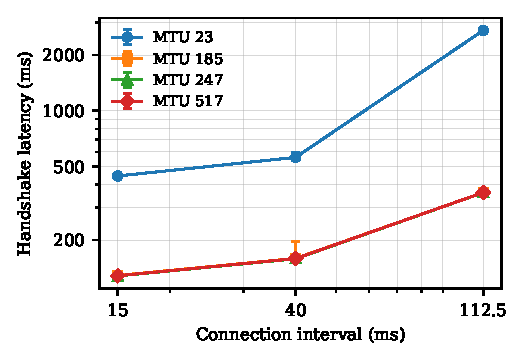
\includegraphics[width=\columnwidth]{figures/fig_latency.pdf}
\caption{Median latency versus connection interval at 240\,MHz (log--log),
with bootstrap 95\% CIs. The curves for MTU 185, 247 and 517\,B overlap.}
\label{fig:latency}
\end{figure}

\subsection{The link dominates}
Table~\ref{tab:latency} and Fig.~\ref{fig:latency} show latency from 3172\,ms
(MTU 23, 112.5\,ms interval, 80\,MHz) down to 128\,ms (MTU $\geq185$, 15\,ms,
240\,MHz), a 24.8$\times$ range. Moving from the default 23\,B MTU to 185\,B
cuts latency by 3.4--8.8$\times$, but larger MTUs add almost nothing: at the
15\,ms interval and 240\,MHz, MTU 185, 247 and 517 give 128.7, 128.0 and
128.3\,ms. With three to seven packets per direction, the handshake fits
in a few connection events, and the event count, not the bytes, sets the
time. At the 112.5\,ms interval every cell with MTU $\geq185$ takes
361\,ms, i.e.\ 3.2 connection intervals, at every clock.

\subsection{When the clock matters}
The ESP32's key generation takes 10.1, 15.0 and 29.8\,ms and decapsulation
13.6, 20.4 and 41.0\,ms at 240, 160 and 80\,MHz. These costs show up only when
the link is fast: at the 15\,ms interval, 80\,MHz is 1.47--1.64$\times$ slower
than 240\,MHz, while at 112.5\,ms the clock changes latency by at most 1.17$\times$
(MTU 23) and not at all for larger MTUs, because the computation finishes
inside the gap between connection events. The phone's encapsulation has a
median of 1.98\,ms over all verified handshakes, so the phone never limits the
handshake.

\begin{figure}[t]
\centering
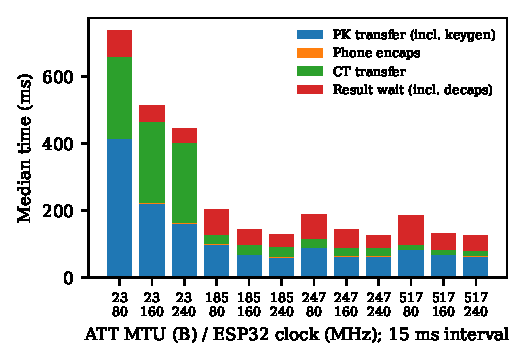
\includegraphics[width=\columnwidth]{figures/fig_phases.pdf}
\caption{Median time per phase at the 15\,ms interval. The PK phase includes
ESP32 key generation; the result wait includes decapsulation.}
\label{fig:phases}
\end{figure}

\subsection{Where the time goes}
Fig.~\ref{fig:phases} splits the handshake. At MTU 23 the CT upload is the
largest phase (239\,ms at 240\,MHz), larger than the PK download (162\,ms)
although the CT is smaller: each of the 55 writes waits for the phone's
Bluetooth stack to accept it. At MTU 517 the CT upload falls to 15\,ms and the
remaining time is the PK phase (64\,ms, of which 10\,ms is key generation)
and the result wait (45\,ms, of which 14\,ms is decapsulation).

\subsection{Phone energy}
Table~\ref{tab:energy} gives the phone's battery current from Android's
\texttt{BatteryManager}, sampled every 50\,ms (the value updated about every
0.4\,s). The whole-phone energy spent while a handshake runs, the product of
current, voltage and median latency, falls from 3278\,mJ at MTU 23 and the
long interval to 140\,mJ at MTU 517 and 15\,ms (240\,MHz). This is dominated
by the phone's baseline draw (224--421\,mA idle with the screen on), so it
tracks latency. The extra current due to the handshake itself could not be
resolved: its 95\% CI was above zero in 9 of 18 cells, below zero in 4 and
spanned zero in 5, because background activity moved the idle current by
more than the handshake added. Measuring the radio's share needs an external
power monitor.

\begin{table}[t]
\centering
\caption{Phone battery current and whole-phone energy per handshake at
240\,MHz. $\Delta I$: handshake minus idle current, block-bootstrap 95\% CI.}
\label{tab:energy}
\footnotesize
\setlength{\tabcolsep}{3pt}
\begin{tabular}{lrrrr}
\toprule
MTU, priority & $I_\mathrm{idle}$ & $I_\mathrm{hs}$ & $\Delta I$ [95\% CI] & $E_\mathrm{phone}$ \\
 & (mA) & (mA) & (mA) & (mJ) \\
\midrule
23, Low power & 322 & 300 & -23 [-70, 16] & 3278 \\
23, Balanced & 240 & 290 & 51 [30, 71] & 652 \\
23, High & 233 & 283 & 49 [33, 66] & 504 \\
517, Low power & 421 & 274 & -146 [-227, -90] & 397 \\
517, Balanced & 224 & 248 & 24 [10, 41] & 157 \\
517, High & 265 & 273 & 8 [-26, 40] & 140 \\
\bottomrule
\end{tabular}

\end{table}

\section{Discussion}
For app developers, the main lever is the link, not the cipher: a 185\,B or
larger MTU and the high connection priority during the handshake bring
ML-KEM-768 to about 130\,ms. Because Android~16 negotiates 517\,B regardless of the request,
peripherals that want a specific MTU must advertise it themselves; most will
get 517\,B and should still cap chunks at 512\,B. On the device side, the
clock is worth raising only when the interval is short; at long intervals a
lower clock costs no latency.

\textit{Limitations:} one phone model, one ESP32 board, one indoor distance
and no interference control; the factorial at MTU 185 and 247\,B came from a
second run on the same day; and energy was measured at the phone only,
through the fuel gauge.

\section{Conclusion}
ML-KEM-768 over BLE between a phone and an ESP32 takes 128\,ms to 3.2\,s,
and the link parameters, not the post-quantum computation, decide where in
that range a product lands. The firmware, app, raw CSVs and analysis are
available at TODO.

\section*{Acknowledgment}
An AI assistant (Claude, Anthropic) was used to help write the firmware,
app and analysis code and to draft and edit the text. The author designed
the study, ran all experiments on the author's own hardware, checked every number
against the measured data, and takes full responsibility for the content.

\bibliographystyle{IEEEtran}
\bibliography{refs}

\end{document}
